\documentclass[11pt, letterpaper]{article}
%basic packages
\usepackage[utf8]{inputenc}
\usepackage[T1]{fontenc}
\usepackage{graphicx}
\usepackage[margin=1in]{geometry}
\usepackage[usenames,dvipsnames]{xcolor}

%math
\usepackage{amsmath, amsthm, amsfonts, amssymb, mathtools}
\usepackage{mathrsfs}
\usepackage{cancel}
\usepackage{siunitx} %phyjsicsssss
\usepackage{bbm} %mathbb for numbers
\usepackage[all]{xy} % https://texdoc.org/serve/xyguide.pdf/0
\makeatletter
\renewcommand*\env@matrix[1][c]{\hskip -\arraycolsep
  \let\@ifnextchar\new@ifnextchar
  \array{*\c@MaxMatrixCols #1}}
\makeatother %matrix realignment

%misc
\usepackage{float}
\usepackage[hyphens]{url}
%\definecolor{page}{HTML}{242526}
%\pagecolor{page}
\usepackage{booktabs} %the \toprule and \bottomrule thick lines on tables
\usepackage{hyperref}

%my commands
\DeclarePairedDelimiter\bra{\langle}{\rvert} %Bra
\DeclarePairedDelimiter\ket{\lvert}{\rangle} %Ket
\DeclarePairedDelimiterX\braket[2]{\langle}{\rangle}{#1\,\delimsize\vert\,\mathopen{}#2} %Bra-ket
\newcommand{\pvec}[1]{\vec{#1}\mkern2mu\vphantom{#1}} % from https://tex.stackexchange.com/questions/120029/how-to-typeset-a-primed-vector
\newcommand{\hati}{\boldsymbol{\hat{\textbf{\i}}}}
\newcommand{\hatj}{\boldsymbol{\hat{\textbf{\j}}}}
\newcommand{\hatk}{\boldsymbol{\hat{\textbf{k}}}}
\newcommand{\R}{\mathbb{R}}
\DeclareMathOperator{\diag}{diag}
\DeclareMathOperator*{\argmax}{arg\,max}
\DeclareMathOperator*{\argmin}{arg\,min}

%theorems
\usepackage{tikz}
\usepackage{tikz-cd}
\usepackage[framemethod=TikZ]{mdframed}
\usepackage{thmtools}
\newtheorem{theorem}{Theorem}
\newtheorem{corollary}{Corollary}
\newtheorem{lemma}{Lemma}
\newtheorem{proposition}{Proposition}

% slightly neater (imo) theorems
%\declaretheoremstyle[headfont=\bfseries, bodyfont=\normalfont, mdframed={linewidth=1pt, bottomline=false, topline=false, rightline=false, leftline=false}]{theorem}
%\declaretheorem[numbered=yes, style=theorem, name=Theorem]{theorem}
%\declaretheorem[numbered=yes, style=theorem, name=Lemma]{lemma}
%\declaretheorem[numbered=yes, style=theorem, name=Corollary]{corollary}
%\declaretheorem[numbered=yes, style=theorem, name=Proposition]{proposition}

% Side Indented Theorems - https://tex.stackexchange.com/questions/429339/shifting-newtheorem
\newtheoremstyle{side}{}{}{\advance\leftskip3cm\relax\itshape\normalfont}{-4pt}
{\bfseries}{}{0pt}{
\makebox[0pt][r]{
  \smash{\parbox[t]{2.5cm}{\raggedright\thmname{#1}.
  \thmnote{\newline(#3)}}}
  \hspace{10.1pt}}}

\theoremstyle{side}
\newtheorem*{note}{Note}
\newtheorem*{intuition}{Intuition}
\newtheorem*{claim}{Claim}
\newtheorem*{prev}{As Previously Seen}

\theoremstyle{definition}
\newtheorem{definition}{Definition}
\newtheorem*{remark}{Remark}
\newtheorem*{example}{Example}
\newtheorem*{notation}{Notation}

\renewcommand{\qedsymbol}{$\blacksquare$}
\declaretheoremstyle[headfont=\bfseries, bodyfont=\normalfont, mdframed={linewidth=1pt, bottomline=false, topline=false, rightline=false, innertopmargin=0pt, innerbottommargin=0pt}, qed=\qedsymbol]{proof}
\declaretheorem[numbered=no, style=proof, name=Proof]{replacementproof}
\renewenvironment{proof}[1][]{\begin{replacementproof}}{\end{replacementproof}}

%fancy headers
\usepackage{fancyhdr}
\pagestyle{fancy}
\fancyhead{}\fancyfoot{}
\fancyfoot[R]{\thepage}
\fancyfoot[C]{\leftmark}

%lectures, taken from (https://castel.dev/post/lecture-notes-3)
\makeatother
\def\@lecture{}%
\newcommand{\lecture}[3]{%
	\ifthenelse{\isempty{#3}}{%

		\def\@lecture{Lecture #1}%
	}{%
		\def\@lecture{Lecture #1: #3}
	}
	\subsection*{\@lecture}
	\hfill{\small\textsf{#2}}\par
}
\makeatletter
\author{Grant Talbert}

\usepackage{titlepageBU}
\title{The Chocolate Bar Game}
\date{10/10/24}
\courseID{MA 293}
\professor{Dr. Borkovitz}
\courseSection{A1}
\begin{document}
\makereport
\newpage
\tableofcontents
\newpage
\vspace*{\fill}
\begin{abstract}
	lol owo
\end{abstract}
\vspace*{\fill}\newpage
\section{Introduction}
The Chocolate Bar Game is a two player game that involves the manipulation of a grid of connected squares, similar to a chocolate bar. Players are allowed to break the grid apart along the lines that run between the squares.

\begin{center}
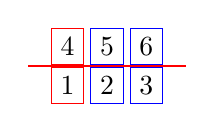
\begin{tikzpicture}
        [square/.style={
            draw,
            minimum width=width("#1"),
            minimum height=width("#1")+2*\pgfshapeinnerysep,
            node contents={#1}}]
	\node at (0,0) (1) [square={$1$}, draw = red];
        \node at (0.5,0) (2) [square={$2$}, draw = blue];
        \node at (1,0) (3) [square={$3$}, draw = blue];
        \node at (0,0.5) (4) [square={$4$}, draw = red];
        \node at (0.5,0.5) (5) [square={$5$}, draw = blue];
        \node at (1,0.5) (6) [square={$6$}, draw = blue];
	\draw [red] (-0.5,0.25) -- (1.5,0.25);
\end{tikzpicture}
\begin{tikzpicture}
	\draw [-{Stealth[length=5mm]}] (0,0) -- node[below=1.6cm] {} (2,0);
\end{tikzpicture}
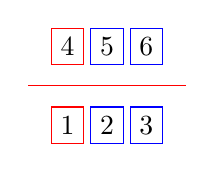
\begin{tikzpicture}
        [square/.style={
            draw,
            minimum width=width("#1"),
            minimum height=width("#1")+2*\pgfshapeinnerysep,
            node contents={#1}}]
	\node at (0,-0.25) (1) [square={$1$}, draw = red];
        \node at (0.5,-0.25) (2) [square={$2$}, draw = blue];
        \node at (1,-0.25) (3) [square={$3$}, draw = blue];
        \node at (0,0.75) (4) [square={$4$}, draw = red];
        \node at (0.5,0.75) (5) [square={$5$}, draw = blue];
        \node at (1,0.75) (6) [square={$6$}, draw = blue];
	\draw [red] (-0.5,0.25) -- (1.5,0.25);
\end{tikzpicture}
\end{center}
\end{document}
